\section{DẤU TAM THỨC BẬC HAI}
\subsection{TÓM TẮT LÝ THUYẾT}
\subsubsection{Dấu của tam thức bậc hai}
\begin{itemize}
	\item [\iconMT] \indam{Định nghĩa:}  Tam thức bậc hai (đối với $x$ ) là biểu thức có dạng $f(x)=ax^2+bx+c$. Trong đó $a, b, c$ là những số cho trước với $a\ne 0$.
	
	\begin{boxkn}
		\begin{itemize}
			\item Nghiệm của phương trình $ax^2+bx+c=0$ được gọi là nghiệm của tam thức bậc hai.
			\item $ \Delta =b^2-4ac$ và $ \Delta '=b'^2-ac$ theo thứ tự được gọi là biệt thức và biệt thức thu gọn của tam thức bậc hai.
		\end{itemize}
	\end{boxkn}
	\item [\iconMT] \indam{Định lý về dấu của tam thức bậc hai: } Ta đã biết hàm số $y=ax^2+bx+c$ với $a \ne 0$ có đồ thị là một parabol.
	\begin{itemize}
		\item [\iconCH] Nếu $a>0$, ta có các trường hợp sau:\\
		\begin{tcolorbox}[colframe=orange,colback=orange!4,boxrule=0.2mm]
				\begin{minipage}{4cm}
				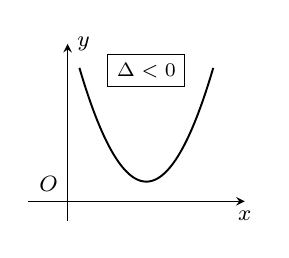
\begin{tikzpicture}[smooth,samples=300,scale=0.5,>=stealth,font=\footnotesize]
					\draw[->] (-1,0)--(4.5,0) node[below]{$x$};
					\draw[->] (0,-0.5)--(0,4) node[right]{$y$};
					\draw (0,0) node[above left]{$O$};
					\draw[line width=0.7pt,domain=0.3:3.7] plot(\x,{(\x)^2-4*(\x)+4.5});
					\node[below] at (2,4) {\fbox{\scriptsize$\Delta <0$}};
				\end{tikzpicture}\\
				\indammm{Đồ thị luôn nằm trên $Ox$.}
			\end{minipage}\hspace{1cm}
			\begin{minipage}{4cm}
				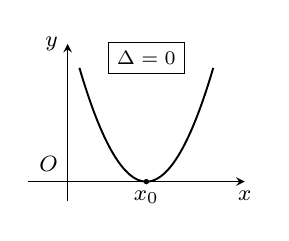
\begin{tikzpicture}[smooth,samples=300,scale=0.5,>=stealth,font=\footnotesize]
					\draw[->] (-1,0)--(4.5,0) node[below]{$x$};
					\draw[->] (0,-0.5)--(0,3.5) node[left]{$y$};
					\draw (0,0) node[above left]{$O$};
					\draw[line width=0.7pt,domain=0.3:3.7] plot(\x,{(\x)^2-4*(\x)+4});
					\draw[fill=black] (2,0) circle(1.5pt);
					\node[below] at (2,0) {$x_0$};
					\node[below] at (2,3.8) {\fbox{\scriptsize$\Delta =0$}};
				\end{tikzpicture}\\
				\indammm{Đồ thị nằm trên $Ox$ khi $x \ne x_0=-\frac{b}{2a}$.}
			\end{minipage}\hspace{1cm}
			\begin{minipage}{4cm}
				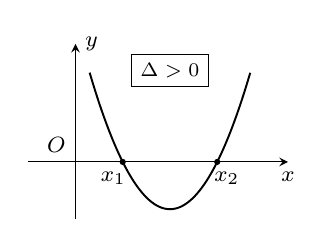
\begin{tikzpicture}[smooth,samples=300,scale=0.6,>=stealth,font=\footnotesize]
					\draw[->] (-1,0)--(4.5,0) node[below]{$x$};
					\draw[->] (0,-1.2)--(0,2.5) node[right]{$y$};
					\draw (0,0) node[above left]{$O$};
					\draw[line width=0.7pt,domain=0.3:3.7] plot(\x,{(\x)^2-4*(\x)+3});
					\draw[fill=black] (1,0) circle(1.5pt) (3,0) circle(1.5pt);
					\node[below] at (0.8,0) {$x_1$};
					\node[below] at (3.2,0) {$x_2$};
					\node[below] at (2,2.5) {\fbox{\scriptsize$\Delta >0$}};
				\end{tikzpicture}\\
				\indammm{Đồ thị nằm trên $Ox$ khi $x<x_1$ hoặc $x>x_2$; nằm dưới $Ox$ khi $x_1<x<x_2$.}
			\end{minipage}
		\end{tcolorbox}
		
		\item [\iconCH] Nếu $a<0$:, ta có các trường hợp sau:\\
		\begin{tcolorbox}[colframe=orange,colback=orange!4,boxrule=0.2mm]
		\begin{minipage}{4cm}
			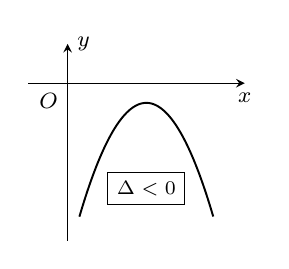
\begin{tikzpicture}[smooth,samples=300,scale=0.5,>=stealth,font=\footnotesize]
				\draw[->] (-1,0)--(4.5,0) node[below]{$x$};
				\draw[->] (0,-4)--(0,1) node[right]{$y$};
				\draw (0,0) node[below left]{$O$};
				\draw[line width=0.7pt,domain=0.3:3.7] plot(\x,{-(\x)^2+4*(\x)-4.5});
				\node[below] at (2,-2) {\fbox{\scriptsize$\Delta <0$}};
			\end{tikzpicture}\\
		\indammm{Đồ thị luôn nằm dưới $Ox$.}
		\end{minipage}\hspace{1cm}
		\begin{minipage}{4cm}
			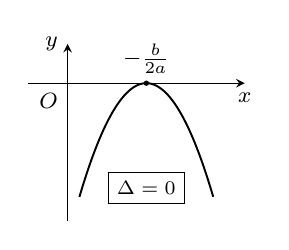
\begin{tikzpicture}[smooth,samples=300,scale=0.5,>=stealth,font=\footnotesize]
				\draw[->] (-1,0)--(4.5,0) node[below]{$x$};
				\draw[->] (0,-3.5)--(0,1) node[left]{$y$};
				\draw (0,0) node[below left]{$O$};
				\draw[line width=0.7pt,domain=0.3:3.7] plot(\x,{-(\x)^2+4*(\x)-4});
				\draw[fill=black] (2,0) circle(1.5pt);
				\node[above] at (2,0) {$-\frac{b}{2a}$};
				\node[below] at (2,-2) {\fbox{\scriptsize$\Delta =0$}};
			\end{tikzpicture}\\
		\indammm{Đồ thị nằm dưới $Ox$ khi $x \ne x_0=-\frac{b}{2a}$.}
		\end{minipage}\hspace{1cm}
		\begin{minipage}{4cm}
			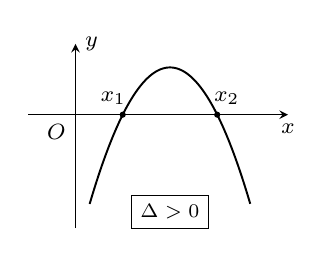
\begin{tikzpicture}[smooth,samples=300,scale=0.6,>=stealth,font=\footnotesize]
				\draw[->] (-1,0)--(4.5,0) node[below]{$x$};
				\draw[->] (0,-2.4)--(0,1.5) node[right]{$y$};
				\draw (0,0) node[below left]{$O$};
				\draw[line width=0.7pt,domain=0.3:3.7] plot(\x,{-(\x)^2+4*(\x)-3});
				\draw[fill=black] (1,0) circle(1.5pt) (3,0) circle(1.5pt);
				\node[above] at (0.8,0) {$x_1$};
				\node[above] at (3.2,0) {$x_2$};
				\node[below] at (2,-1.5) {\fbox{\scriptsize$\Delta >0$}};
			\end{tikzpicture}\\
		\indammm{Đồ thị nằm dưới $Ox$ khi $x<x_1$ hoặc $x>x_2$; nằm trên $Ox$ khi $x_1<x<x_2$.}
		\end{minipage}
		\end{tcolorbox}
	\end{itemize}
\end{itemize}
Tương ứng hình ảnh đồ thị ở trên, ta có bảng tổng kết dấu của tam thức bậc hai như sau:
\begin{itemize}
	\item [\iconCH] Nếu $a>0$:
	\begin{listEX}[3]
		\item [] 
\begin{tikzpicture}[scale=0.8,font=\footnotesize]
			\tkzTabInit[nocadre=false,lgt=1,espcl=2.5]
			{$x$ /0.6,$f(x)$ /0.6}
			{$-\infty$,$+\infty$}
			\tkzTabLine{,+,}
		\end{tikzpicture}
		\item [] 
\begin{tikzpicture}[scale=0.8,font=\footnotesize]
			\tkzTabInit[nocadre=false,lgt=1,espcl=1.4]
			{$x$ /0.6,$f(x)$ /0.6}
			{$-\infty$,$x_0$,$+\infty$}
			\tkzTabLine{,+,$0$,+,}
		\end{tikzpicture}
		\item [] 
\begin{tikzpicture}[scale=0.8,font=\footnotesize]
			\tkzTabInit[nocadre=false,lgt=1,espcl=1.2]
			{$x$ /0.6,$f(x)$ /0.6}
			{$-\infty$,$x_1$,$x_2$,$+\infty$}
			\tkzTabLine{,+,$0$,-,$0$,+,}
		\end{tikzpicture}
	\end{listEX}
	\item [\iconCH] Nếu $a<0$:
	\begin{listEX}[3]
		\item [] 
\begin{tikzpicture}[scale=0.8,font=\footnotesize]
			\tkzTabInit[nocadre=false,lgt=1,espcl=2.5]
			{$x$ /0.6,$f(x)$ /0.6}
			{$-\infty$,$+\infty$}
			\tkzTabLine{,-,}
		\end{tikzpicture}
		\item [] 
\begin{tikzpicture}[scale=0.8,font=\footnotesize]
			\tkzTabInit[nocadre=false,lgt=1,espcl=1.4]
			{$x$ /0.6,$f(x)$ /0.6}
			{$-\infty$,$x_0$,$+\infty$}
			\tkzTabLine{,-,$0$,-,}
		\end{tikzpicture}
		\item [] 
\begin{tikzpicture}[scale=0.8,font=\footnotesize]
			\tkzTabInit[nocadre=false,lgt=1,espcl=1.2]
			{$x$ /0.6,$f(x)$ /0.6}
			{$-\infty$,$x_1$,$x_2$,$+\infty$}
			\tkzTabLine{,-,$0$,+,$0$,-,}
		\end{tikzpicture}
	\end{listEX}
\end{itemize}
\newpage
\begin{minipage}{8cm}
	\begin{tcolorbox}[colframe=cyan,colback=cyan!3,boxrule=0.2mm]
		\indamm{Định lý về dấu tam thức bậc hai:} Cho tam thức bậc hai $f(x)=ax^2+b x+c\,(a \neq 0)$.
		\begin{itemize}
			\item [\iconCH] Nếu $\Delta<0$ thì $f(x)$ cùng dấu với hệ số $a$ với mọi $x \in \mathbb{R}$.
			\item [\iconCH] Nếu $\Delta=0$ thì $f(x)$ cùng dấu với hệ số $a$ với mọi $x \neq-\frac{b}{2 a}$.
			\item [\iconCH] Nếu $\Delta>0$ thì tam thức $f(x)$ có hai nghiệm phân biệt $x_1$ và $x_2$ $\left(x_{1}<x_{2}\right)$. Khi đó, $f(x)$ cùng dấu với hệ số $a$ với mọi $x \in\left(-\infty ; x_{1}\right) \cup\left(x_{2} ;+\infty\right) ; f(x)$ trái dấu với hệ số $a$ với mọi $x \in\left(x_{1} ; x_{2}\right)$
		\end{itemize}
	\end{tcolorbox}
\end{minipage}\hspace{0.5cm}
\begin{minipage}{9cm}
\begin{khung4}{Ghi nhớ dấu của $f(x)$ và $a$}
\begin{itemize}
	\item[\iconCH] Nếu $\Delta < 0$ thì\\
		\begin{tikzpicture}
			\tkzTabInit[nocadre=false,lgt=1.2,espcl=4.2]
			{$x$ /0.7,$f(x)$ /0.8}
			{$-\infty$,$+\infty$}
			\tkzTabLine{,\text{cùng dấu },}
		\end{tikzpicture}
	\item[\iconCH] Nếu $\Delta = 0$ thì\\
		\begin{tikzpicture}
			\tkzTabInit[nocadre=false,lgt=1.2,espcl=2.5]
			{$x$ /0.7,$f(x)$ /0.8}
			{$-\infty$,$-\frac{b}{2a}$,$+\infty$}
			\tkzTabLine{,\text{cùng dấu },$0$,\text{ cùng dấu },}
		\end{tikzpicture}
	\item[\iconCH] Nếu $\Delta > 0$ thì\\
		\begin{tikzpicture}
		\tkzTabInit[nocadre=false,lgt=1.2,espcl=1.7]
		{$x$ /0.7,$f(x)$ /1}
		{$-\infty$,$x_1$,$x_2$,$+\infty$}
		\tkzTabLine{,\text{cùng dấu },$0$,\text{ trái dấu },$0$,\text{ cùng dấu },}
	\end{tikzpicture}
\end{itemize}
\end{khung4}
\end{minipage}

\subsubsection{Bất phương trình bậc hai}
\begin{itemize}
	\item [\iconMT] \indam{Định nghĩa:} Bất phương trình bậc hai ẩn $x$ là bất phương trình có dạng $a x^{2}+b x+c>0$ (hoặc $\left.a x^{2}+b x+c \geq 0, a x^{2}+b x+c<0, a x^{2}+b x+c \leq 0\right)$, trong đó $a, b, c$ là những số thực đã cho và $a \neq 0$.
	\item [\iconMT] \indam{Một số kết quả cần nhớ:} Cho tam thức bậc hai $ax^2+bx+c$, với $a \ne 0$.
	\begin{listEX}[2]
		\item [\ding{172}]$ax^2+bx+c>0, \forall x\in \mathbb{R} \Leftrightarrow \left\{\begin{aligned}
			&a>0\\
			& \Delta <0.
		\end{aligned}\right.$
		\item [\ding{173}] $ax^2+bx+c<0, \forall x\in \mathbb{R} \Leftrightarrow \left\{\begin{aligned}
			&a<0\\
			& \Delta <0.
		\end{aligned}\right. $
		\item [\ding{174}] $ax^2+bx+c\geqslant 0, \forall x\in \mathbb{R} \Leftrightarrow \left\{\begin{aligned}
			&a>0\\
			& \Delta \leqslant 0.
		\end{aligned}\right. $
		\item [\ding{175}] $ax^2+bx+c\leqslant 0, \forall x\in \mathbb{R} \Leftrightarrow \left\{\begin{aligned}
			&a<0\\
			& \Delta \leqslant 0.
		\end{aligned}\right. $
	\end{listEX}
\end{itemize}

\subsection{RÈN LUYỆN KĨ NĂNG GIẢI TOÁN}
\begin{dang}{Xét dấu tam thức bậc hai $f(x)=ax^2+bx+c$, với $a \ne 0$}
	\begin{itemize}
		\item [$\bullet$] Tìm nghiệm $ax^2+bx+c=0 \quad (1)$.
		\item [$\bullet$] Tùy thuộc vào số nghiệm của (1), ta lựa chọn bảng xét dấu phù hợp.
	\end{itemize}
\begin{note}
	Ghi nhớ ngắn gọn: Nếu $\Delta \le 0$ thì cùng dấu $a$; Nếu $\Delta >0 $ thì  "trong trái, ngoài cùng".
\end{note}
\end{dang}

\begin{vd}%[0D4Y5-1]
	Xét dấu của các tam thức sau
	\begin{listEX}[3]
		\item $3x^2-2x+1$.
		\item $-x^2+4x+5$.
		\item $4x^2+4x+1$.
		\item $2x^2 - 6x + 4{,}5$.
		\item $3x^2 - 2x - 8$ .
		\item $- x^2 + 2x - 1$.
	\end{listEX}
	\loigiai{
		\begin{listEX}
			\item Ta có $ \Delta '=-2<0$ và $a=3>0$. Suy ra $3x^2-2x+1>0,\forall x\in \mathbb{R}$.
			\item Ta có $-x^2+4x+5=0 \Leftrightarrow \left[\begin{aligned}& x=-1 \\ & x=5.\end{aligned}\right. $\\
			Bảng xét dấu
			\begin{center}
				
\begin{tikzpicture}
					\tkzTabInit[lgt=3,espcl=2]
					{$x$ /0.8, $-x^2+4x+5$ /0.8}
					{$-\infty$,$-1$,$5$,$+\infty$}
					\tkzTabLine{ ,-,$0$,+,$0$,-,}
				\end{tikzpicture}
			\end{center}
			Suy ra $-x^2+4x+5>0 \Leftrightarrow x\in (-1;5)$ và $-x^2+4x+5<0 \Leftrightarrow x\in (-\infty;-1)\cup (5;+\infty)$.
			\item Tam thức bậc hai $f(x)=4x^2+4x+1$ có $\Delta=0$, nghiệm kép $x_0=-\dfrac{1}{2}$ và hệ số $a=4>0$ nên $f(x)>0$ với mọi $x\in\mathbb{R}\setminus\left\{-\dfrac{1}{2}\right\}$.
			\item Ta có $f(x)=0\Leftrightarrow 2x^2-6x+\dfrac{9}{2}=0\Leftrightarrow x=\dfrac{3}{2}$.\\ Bảng xét dấu
			\begin{center}
				
\begin{tikzpicture}
					\tkzTabInit[nocadre=false,lgt=1.2,espcl=4,deltacl=0.6] %phần bắt buộc
					{$x$ /1,$f(x)$ /0.6}
					{$-\infty$,$\dfrac{3}{2}$,$+\infty$}
					\tkzTabLine{,+,$0$,+,}
				\end{tikzpicture}
			\end{center}
			\item Ta có $f(x)=0\Leftrightarrow 3x^2-2x-8=0\Leftrightarrow \hoac{& x=-\dfrac{4}{3} \\ & x=2}$.\\ Bảng xét dấu
			\begin{center}
				
\begin{tikzpicture}
					\tkzTabInit[nocadre=false,lgt=1.2,espcl=2.5,deltacl=0.6] %phần bắt buộc
					{$x$ /1,$f(x)$ /0.6}
					{$-\infty$,$-\dfrac{4}{3}$,$2$,$+\infty$}
					\tkzTabLine{,+,$0$,-,$0$,+,}
				\end{tikzpicture}
			\end{center}
			\item Ta có $f(x)=0\Leftrightarrow -x^2+2x-1=0\Leftrightarrow x=1$.\\ Bảng xét dấu
			\begin{center}
				
\begin{tikzpicture}
					\tkzTabInit[nocadre=false,lgt=1.2,espcl=4,deltacl=0.6] %phần bắt buộc
					{$x$ /1,$f(x)$ /0.6}
					{$-\infty$,$1$,$+\infty$}
					\tkzTabLine{,-,$0$,-,}
				\end{tikzpicture}
			\end{center}
		\end{listEX}
	}
\end{vd}\dongcham{21}
\begin{vd}%[0D4B5-1]
	Tìm nghiệm và lập bảng xét dấu của tam thức bậc hai $f(x)$ với đồ thị được cho ở mỗi hình\\
	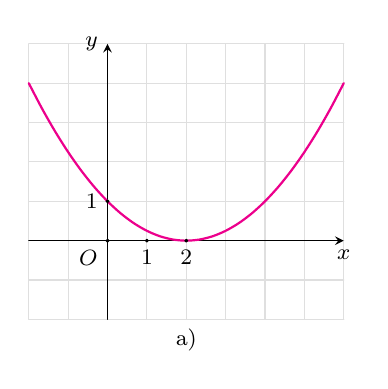
\begin{tikzpicture}[scale=.5, font=\footnotesize, line join=round, line cap=round, >=stealth]
		\draw[gray!50,opacity=.5](-2,-2)grid(6,5);
		\draw[->](-2,0)--(0,0)node[below left]{$O$}--(6,0)node[below]{$x$};
		\draw[->](0,-2)--(0,5)node[left]{$y$};
		\draw[smooth,domain=-2:6,thick,magenta]plot(\x,{1/4*(\x)^2-(\x)+1});
		\draw (2,-2)node[below]{a)};
		\draw(1,0)node[below]{$1$};
		\draw(2,0)node[below]{$2$};
		\draw(0,1)node[left]{$1$};
		\foreach \x in{0,1,2}\draw[fill](\x,0)circle(1pt);
		\draw[fill](0,1)circle(1pt);
		
	\end{tikzpicture}\hspace*{1cm}
	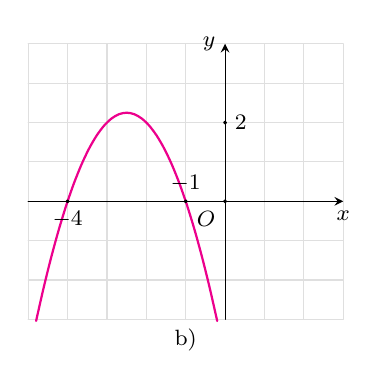
\begin{tikzpicture}[scale=.5, font=\footnotesize, line join=round, line cap=round, >=stealth]
		\draw[gray!50,opacity=.5](-5,-3)grid(3,4);
		\draw[->](-5,0)--(0,0)node[below left]{$O$}--(3,0)node[below]{$x$};
		\draw[->](0,-3)--(0,4)node[left]{$y$};
		\draw[smooth,domain=-4.8:-0.2,thick,magenta]plot(\x,{-(\x)^2-5*(\x)-4});
		\draw (-1,-3)node[below]{b)};
		\draw(-4,0)node[below]{$-4$};
		\draw(0,2)node[right]{$2$};
		\draw(-1,0)node[above]{$-1$};
		\foreach \x in{-4,-1,0}\draw[fill](\x,0)circle(1pt);
		\draw[fill](0,2)circle(1pt);
		
	\end{tikzpicture}\hspace*{1cm}
	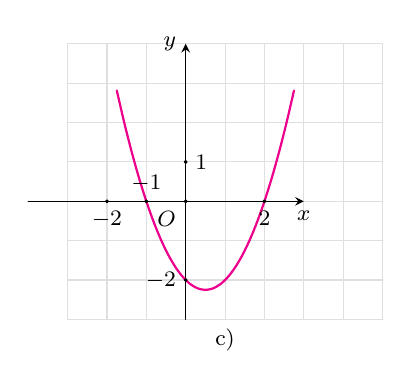
\begin{tikzpicture}[scale=.5, font=\footnotesize, line join=round, line cap=round, >=stealth]
		\draw[gray!50,opacity=.5](-3,-3)grid(5,4);
		\draw[->](-4,0)--(0,0)node[below left]{$O$}--(3,0)node[below]{$x$};
		\draw[->](0,-3)--(0,4)node[left]{$y$};
		\draw[smooth,domain=-1.75:2.75,thick,magenta]plot(\x,{(\x)^2-(\x)-2});
		\draw (1,-3)node[below]{c)};
		\draw(0,1)node[right]{$1$};
		\draw(0,-2)node[left]{$-2$};
		\draw(-2,0)node[below]{$-2$};
		\draw(-1,0)node[above]{$-1$};
		\draw(2,0)node[below]{$2$};
		\foreach \x in {-2,-1,0,2}\draw[fill](\x,0)circle(1pt);
		\foreach \x in {-2,1}\draw[fill](0,\x)circle(1pt);
		
	\end{tikzpicture}
	\loigiai{
		\begin{enumEX}[a)]{1}
			\item \immini{Từ đồ thị hình a) ta có nghiệm của tam thức bậc hai $f(x)$ là $x=2$. Bảng xét dấu của tam thức là}{
				
\begin{tikzpicture}
					\tkzTabInit[deltacl=0.6,espcl=2.5,lgt=2,nocadre=false]
					{$x$/0.6,$f(x)$/0.6}
					{$-\infty$,$2$,$+\infty$}
					\tkzTabLine{,+,0,+,}
					
				\end{tikzpicture}
			}
			\item \immini{Từ đồ thị hình b) ta có tam thức bậc hai $f(x)$ có $2$ nghiệm $x_1=-4$ và $x_2=-1$. Bảng xét dấu của tam thức là}{
				
\begin{tikzpicture}
					\tkzTabInit[deltacl=0.6,espcl=2.5,lgt=2,nocadre=false]
					{$x$/0.6,$f(x)$/0.6}
					{$-\infty$,$-4$,$-1$,$+\infty$}
					\tkzTabLine{,-,0,+,0,-,}
					
				\end{tikzpicture}
			}
			\item \immini{Từ đồ thị hình c) ta có nghiệm của tam thức bậc hai $f(x)$ là $x_1=-1$ và $x_2=2$. Bảng xét dấu của tam thức là}{
				
\begin{tikzpicture}
					\tkzTabInit[deltacl=0.6,espcl=2.5,lgt=2,nocadre=false]
					{$x$/0.6,$f(x)$/0.6}
					{$-\infty$,$-1$,$2$,$+\infty$}
					\tkzTabLine{,+,0,-,0,+,}
					
				\end{tikzpicture}
			}
		\end{enumEX}
	}
\end{vd}\dongcham{14}

\begin{dang}{Giải bất phương trình bậc hai}
	Ta lập bảng xét dấu của tam thức bậc hai. Sau đó, chọn  kết quả phù hợp với yêu cầu đề bài.
\end{dang}
\begin{vd}%[0D4Y5-2]
	Giải các bất phương trình sau	
	\begin{listEX}[3]
		\item $-3x^2+2x+1<0$.
		\item $x^2+x-12\ge 0$.
		\item $-x^2+x+6 \le 0$.
		\item $-x^2+x-5<0$
		\item $x^2-2x-4>0$
		\item $4x^2+4x+1>0$
	\end{listEX}
	\loigiai{
		\begin{listEX}
			\item Ta có $-3x^2+2x+1=0 \Leftrightarrow x=-\dfrac{1}{3}$ hoặc $x=1$.\\
			Bảng xét dấu
			\begin{center}
				
\begin{tikzpicture}
					\tkzTabInit[lgt=3,espcl=2]
					{$x$ /1.2, $-x^2+4x+5$ /0.8}
					{$-\infty$,$-\dfrac{1}{3}$,$1$,$+\infty$}
					\tkzTabLine{ ,-,$0$,+,$0$,-,}
				\end{tikzpicture}
			\end{center}
			Dựa vào bảng xét dấu, ta có tập nghiệm của bất phương trình là $S=\left(-\infty;-\dfrac{1}{3}\right)\cup (1;+\infty)$.
			\item Ta có $x^2+x-12=0 \Leftrightarrow x=3$ hoặc $x=-4$.\\
			Bảng xét dấu
			\begin{center}
				
\begin{tikzpicture}
					\tkzTabInit[lgt=3,espcl=2]
					{$x$ /0.8, $x^2+x-12$/0.8}
					{$-\infty$,$-4$,$3$,$+\infty$}
					\tkzTabLine{ ,+,$0$,-,$0$,+,}
				\end{tikzpicture}
			\end{center}
			Dựa vào bảng xét dấu, ta có tập nghiệm của bất phương trình là $S=(-\infty;-4] \cup [3;+\infty)$.	
			\item Ta có $-x^2+x+6=0 \Leftrightarrow x=-2$ hoặc $x=3$.
			Bảng xét dấu
			\begin{center}
				
\begin{tikzpicture}
					\tkzTabInit[lgt=3,espcl=2]
					{$x$ /1.2, $-x^2+x+6$ /0.8}
					{$-\infty$,$-2$,$3$,$+\infty$}
					\tkzTabLine{ ,-,$0$,+,$0$,-,}
				\end{tikzpicture}
			\end{center}
			Dựa vào bảng xét dấu, ta có tập nghiệm của bất phương trình là $S=\left(-\infty;-2\right]\cup [3;+\infty)$.
			\item $-x^2+x-5=0$ vô nghiệm nên ta có bảng xét dấu
			\begin{center}
				
\begin{tikzpicture}
					\tkzTabInit[lgt=3,espcl=2]
					{$x$ /0.8, $-x^2+x-5$ /0.8}
					{$-\infty$,$+\infty$}
					\tkzTabLine{ ,-,}
				\end{tikzpicture}
			\end{center}
			Dựa vào bảng xét dấu, ta có tập nghiệm của bất phương trình là $\mathbb{R}$.
			\item Ta có $x^2-2x-4>0\Leftrightarrow x\in\left(-\infty;1-\sqrt{5}\right)\cup \left(1+\sqrt{5};+\infty\right)$.
			\item Ta có $4x^2+4x+1=0\Leftrightarrow x=-\dfrac{1}{2} $.\\
			Bảng xét dấu
			\begin{center}
				
\begin{tikzpicture}
					\tkzTabInit[lgt=3,espcl=2]
					{$x$ /1.2, $4x^2+4x+1$ /0.8}
					{$-\infty$,$-\frac{1}{2}$,$+\infty$}
					\tkzTabLine{ ,+,$0$,+,}
				\end{tikzpicture}
			\end{center}
			Tập nghiệm của bất phương trình là $\mathbb{R}\setminus\left\{-\dfrac{1}{2}\right\}$.
			
		\end{listEX}
	}
\end{vd}\dongcham{25}
\begin{vd}
	Tìm nghiệm của bất phương trình $ax^2+bx+c>0$, với đồ thị $f(x)=ax^2+bx+c$ được cho ở mỗi hình bên:\\
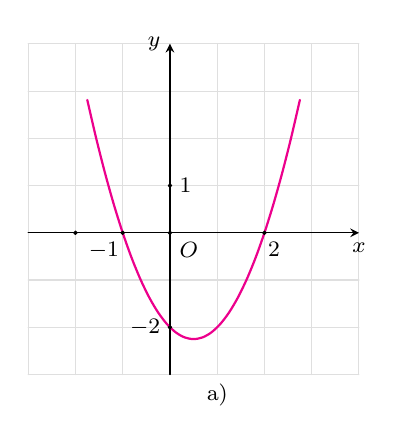
\begin{tikzpicture}[scale=.6, font=\footnotesize, line join=round, line cap=round, >=stealth]
	\draw[gray!50,opacity=.5](-3,-3)grid(4,4);
	\draw[->](-3,0)--(0,0)node[below right]{$O$}--(4,0)node[below]{$x$};
	\draw[->](0,-3)--(0,4)node[left]{$y$};
	\draw[smooth,domain=-1.75:2.75,thick, magenta]plot(\x,{(\x)^2-(\x)-2});
	\draw (1,-3)node[below]{a)};
	\draw(0,1)node[right]{$1$};
	\draw(0,-2)node[left]{$-2$};
	\draw(-1.4,0)node[below]{$-1$};
	\draw(2.2,0)node[below]{$2$};
	\foreach \x in {-2,-1,0,2}\draw[fill](\x,0)circle(1pt);
	\foreach \x in {-2,1}\draw[fill](0,\x)circle(1pt);
\end{tikzpicture}\hspace{1cm}
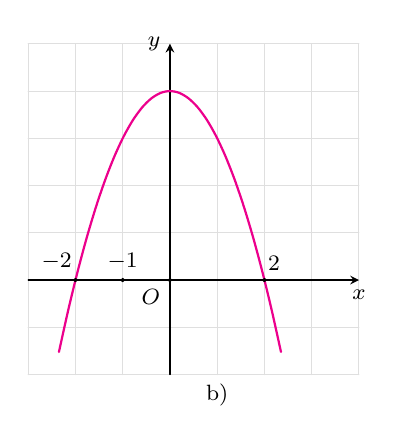
\begin{tikzpicture}[scale=.6, font=\footnotesize, line join=round, line cap=round, >=stealth]
	\draw[gray!50,opacity=.5](-3,-2)grid(4,5);
	\draw[->](-3,0)--(0,0)node[below left]{$O$}--(4,0)node[below]{$x$};
	\draw[->](0,-2)--(0,5)node[left]{$y$};
	\draw[smooth,domain=-2.35:2.35,thick, magenta]plot(\x,{-(\x)^2+4});
	\draw (1,-2)node[below]{b)};
	\draw(-2.4,0)node[above]{$-2$};
	\draw(-1,0)node[above]{$-1$};
	\draw(2.2,0)node[above]{$2$};
	\foreach \x in {-2,-1,0,2}\draw[fill](\x,0)circle(1pt);
\end{tikzpicture}\hspace{1cm}
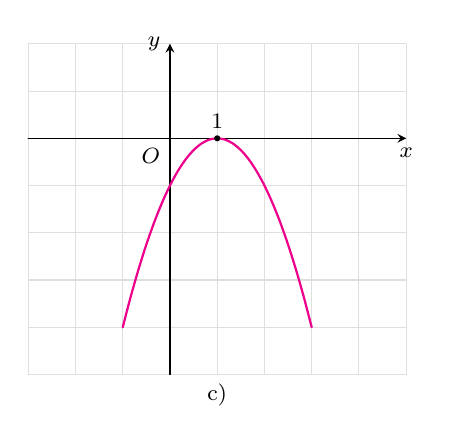
\begin{tikzpicture}[scale=.6, font=\footnotesize, line join=round, line cap=round, >=stealth]
	\draw[gray!50,opacity=.5](-3,-5)grid(5,2);
	\draw[->](-3,0)--(0,0)node[below left]{$O$}--(5,0)node[below]{$x$};
	\draw[->](0,-5)--(0,2)node[left]{$y$};
	\draw[smooth,domain=-1:3,thick, magenta]plot(\x,{-(\x-1)^2});
	\draw (1,-5)node[below]{c)};
	\draw(1,0)node[above]{$1$};
	\foreach \x in {1}\draw[fill](\x,0)circle(1.5pt);
\end{tikzpicture}
	\loigiai{}
\end{vd}\dongcham{20}
\begin{dang}{Vận dụng, thực tiễn}
\end{dang}

\begin{vd}
	Tìm các giá trị của tham số $m$ để 
	\begin{enumEX}[a)]{2}
		\item $x^2 - 2x + m \geq 0,\, \forall x\in  \mathbb{R}$.
		\item $x^2 -2mx + 4- 3m>0,\, \forall x\in  \mathbb{R} $. 
		\item $-x^2 -2 (2m-1) x+ 1 -2m \le 0,\, \forall x\in  \mathbb{R} $. 
		\item $-2x^2+2(m-2)x+m-2<0,\, \forall x\in  \mathbb{R} $. 
	\end{enumEX}
	\loigiai{
		\begin{itemize}
			\item [a)] Bất phương trình thỏa mãn với mọi số thực thì $\Delta \leq 0 \ (\Delta' \leq 0)$.\\
			$\Delta' = (-1)^2 - m \leq 0 \Leftrightarrow m \geq 1$.
			\item [b)] Ta có $\Delta '= b'^2 -a c = m^2 + 3m-4$.\\
			Khi đó $P(x) >0 $ $\forall x \Leftrightarrow \heva{& a > 0\\& \Delta ' <0 } \Leftrightarrow \heva{& 1 >0 \text{ (luôn đúng)}\\& m^2 + 3m -4 < 0} \Leftrightarrow m^2 + 3m -4 <0$.\\
			Bảng xét dấu \\
			\begin{center}
				
\begin{tikzpicture}
					\tkzTabInit
					[lgt=2.5,espcl=2] % tùy chọn
					{$m $/1, $m^2 + 3m -4 $/1.3} % cột 1
					{$-\infty $,$-4$,$1$,$+ \infty $} % hàng 1 cột 2
					\tkzTabLine{, +  , z , - , z , + , } % hàng 2 cột 2
				\end{tikzpicture}
			\end{center}
			Dựa vào bảng xét dấu ta thấy $m \in (-4;1)$ thoả mãn yêu cầu bài toán.
			\item [c)] Ta có $\Delta ' = b'^2 - ac = (2m-1)^2 + (1-2m) = 4m^2 -6m +2. $\\
			Khi đó $P(x) \le 0$ $\forall x \Leftrightarrow \heva{&a <0 \\& \Delta ' \le 0} \Leftrightarrow \heva{&-1<0 \text{ (luôn đúng)} \\& 4m^2 - 6m+2 \le 0} \Leftrightarrow 4m^2 - 6m+2 \le 0. $\\
			Bảng xét dấu \\
			\begin{center}
				
\begin{tikzpicture}
					\tkzTabInit
					[lgt=3 ,espcl=2] % tùy chọn
					{$m$/1, $4m^2 -6m +2  $/1.3} % cột 1
					{$-\infty $,$\dfrac{1}{2}$,$1$,$+ \infty $} % hàng 1 cột 2
					\tkzTabLine{, +  , z , - , z , + , } % hàng 2 cột 2
				\end{tikzpicture}
			\end{center}
			Dựa vào bảng xét dấu ta thấy $m \in \left[ \dfrac{1}{2};1\right]$ thoả mãn yêu cầu bài toán.
			\item [d)] Yêu cầu bài toán tương đương với
			{\allowdisplaybreaks
				\begin{eqnarray*}
					&&f(x)=-2x^2+2(m-2)x+m-2\le 0,\forall x\in\mathbb{R} \\
					&\Leftrightarrow & \Delta' =(m-2)^2+2\cdot(m-2)< 0\\
					&\Leftrightarrow & m(m-2)< 0\\
					&\Leftrightarrow & 0< m< 2.
			\end{eqnarray*}}
			Vậy, giá trị cần tìm của $m$ là $0< m< 2$.
		\end{itemize}
	}
\end{vd}\dongcham{16}

\begin{vd}
	Độ cao so với mặt đất của một quả bóng được ném lên theo phương thẳng đứng được mô tả bởi hàm số bậc hai $h(t)=-4,9 t^{2}+20 t+1$, ở đó độ cao $h(t)$ tính bằng mét và thời gian $t$ tính bằng giây. Trong khoảng thời điểm nào trong quá trình bay của nó, quả bóng sẽ ở độ cao trên $5$ m so với mặt đất?
	\loigiai{
		Xét bất phương trình $$-4,9 t^{2}+20 t+1>5\Leftrightarrow-4,9 t^{2}+20 t-4>0$$
		Nghiệm của phương trình
		$-4,9 t^{2}+20 t-4=0$ là $t \approx 0,21 ; t \approx 3,87$.
		Do đó, nghiệm của bất phương trình là $t \in(0,21 ; 3,87)$. Vậy khoảng thời điểm $t \in(0,21 ; 3,87)$
		(s) trong quá trình bay của quả bóng thì nó sẽ ở độ cao trên $5 \mathrm{~m}$ so với mặt đất.}
\end{vd}\dongcham{12}

\begin{vd}
	Một vật được ném theo phương thẳng đứng xuống dưới từ độ cao $320 \mathrm{~m}$ với vận tốc ban đầu $v_{Q}=20 \mathrm{~m} / \mathrm{s}$. Hỏi sau ít nhất bao nhiêu giây, vật đó cách mặt đất không quá $100 \mathrm{~m}$ ? Giả thiết rằng sức cản của không khí là không đáng kể.
	\loigiai{
		Độ cao của vật so với mặt đất được cho bởi công thức
		$$
		h(t)=h_{0}+v_{0} t-\frac{1}{2} g t^{2}=320+20 t-4,9 t^{2}(\mathrm{~m}) .
		$$
		Vật cách mặt đất không quá $100 \mathrm{~m}$ khi và chỉ khi $h(t) \leq 100$, tức là $-4,9 t^{2}+20 t+320 \leq 100$ hay tương đương $4,9 t^{2}-20 t-220 \geq 0$.\\
		Giải bất phương trình này và chú ý đến điều kiện $t>0$ ta được: $t \geq \frac{10+\sqrt{1178}}{4,9} \approx 9,05(\mathrm{~s})$.
	}
\end{vd}\dongcham{13}

\begin{vd}
	\immini{Xét đường tròn đường kính $AB=4$ và một điểm $M$ di chuyển trên đoạn $A B$, đặt $A M=x$. Xét hai đường tròn đường kính $A M$ và $M B$. Kí hiệu $S(x)$ là diện tích phần hình phẳng nằm trong hình tròn lớn và nằm ngoài hai hình tròn nhỏ. Xác định các giá trị của $x$ để diện tích $S(x)$ không vượt quá một nửa tổng diện tích hai hình tròn nhỏ.}{
		\begin{tikzpicture}[smooth,font=\footnotesize,scale=1,>=latex]
			\path
			(0,0) coordinate (A)
			(4,0) coordinate (B)
			(1.5,0) coordinate (M)
			($(A)!0.5!(B)$)coordinate (O)
			($(A)!0.5!(M)$)coordinate (O1)
			($(M)!0.5!(B)$)coordinate (O2)
			($(A)+(0,3)$)coordinate (X)
			($(A)+(0,2.3)$)coordinate (X')
			($(B)+(0,3)$)coordinate (Y)
			($(M)+(0,2.3)$)coordinate (Y')
			;
			\fill[cyan] (O) circle (2);
			\fill[white] (O1) circle (0.75);
			\fill[white] (O2) circle (1.25);
			\draw 
			(O) circle (2)
			(O1) circle (0.75)
			(O2) circle (1.25);
			\draw[dashed,<->](X)--(Y)node[above,midway,sloped,scale=.8]{$4$ };
			\draw[dashed,<->](X')--(Y')node[above,midway,sloped,scale=.8]{$x$ };
			\draw[dashed](A)--(X) (B)--(Y) (M)--(Y');
			\draw(A)node[left]{$A$}--(M)node[below right]{$M$}--(B)node[right]{$B$};
			%\path (A)--(M1) node[below,midway,sloped,scale=.8]{\scriptsize $3,2$m }
	\end{tikzpicture}}
	\loigiai{
		Vì điểm $M$ nằm giữa $A$ và $B$ nên $M B=A B-A M=4-x$.
		Gọi $S, S_{1}, S_{2}$ lần lượt là diện tích hình tròn đường kính $A B, A M$ và $M B$.
		Ta có: $\quad S_{1}+S_{2}=\pi\left(\frac{x}{2}\right)^{2}+\pi\left(\frac{4-x}{2}\right)^{2}=\frac{x^{2}-4 x+8}{2} \pi$.
		$$
		S(x)=S-\left(S_{1}+S_{2}\right)=4 \pi-\frac{x^{2}-4 x+8}{2} \pi=\frac{-x^{2}+4 x}{2} \pi .
		$$
		Do đó từ điều kiện $S(x) \leq \frac{1}{2}\left(S_{1}+S_{2}\right)$ ta được bất phương trình bậc hai $3 x^{2}-12 x+8 \geq 0$.
		Giải bất phương trình bậc hai này và kết hợp với điều kiện $0 \leq x \leq 4$, ta được
		$$
		x \in\left[0 ; \frac{6-2 \sqrt{3}}{3}\right] \cup\left[\frac{6+2 \sqrt{3}}{3} ; 4\right]
		$$}
\end{vd}\dongcham{15}

\begin{vd}%
	\immini{Một tình huống trong huấn luyện pháo binh được mô tả như sau: Trong mặt phẳng tọa độ $Oxy$, khẩu đại bác được biểu thị bằng điểm $O(0; 0)$ và bia mục tiêu được biểu thị bằng đoạn thẳng $MN$ với $M(2100; 25)$ và $N(2100; 15)$ (Hình 29). Xạ thủ cần xác định parabol $y=-a^2x^2+10ax$ $(a>0)$ mô tả quỹ đạo chuyển động của viên đạn sao cho viên đạn bắn ra từ khẩu đại bác phải chạm vào bia mục tiêu. Tìm giá trị lớn nhất của $a$ để xạ thủ đạt được mục đích trên.
	}{\begin{tikzpicture}[scale=1, font=\footnotesize, line join=round, line cap=round, >=stealth]
			\def\a{-.25} \def\b{1} \def\c{0} % Hệ số
			\def\xt{-1} \def\xp{6} \def\yt{3} \def\yd{-1} % x_trái, x_phải, y_trên, y_dưới (giới hạn)
			\draw[->] (\xt,0)--(\xp,0) node [below]{$x$};
			\draw[->] (0,\yd)--(0,\yt) node [left]{$y$};
			\node at (0,0) [below left]{$O$};
			\clip (\xt-0.1,\yd+0.1) rectangle (\xp-0.1,\yt-0.1);
			\draw[smooth,samples=300,domain=0:4] plot(\x,{\a*(\x)^2+\b*(\x)+\c});
			\draw[fill=black] (3,0) node[shift={(-90:.4)}]{$2100$} circle(1pt);
			\draw[fill=black] (3,1) node[shift={(90:.4)}]{$M$} circle(1pt);
			\draw[fill=black] (3,.5) node[shift={(180:.3)}]{$N$} circle(1pt);
			\draw[line width=2pt] (3,1)--(3,.5);
			\draw (2,1) node[shift={(90:1)}]{$y=-a^2x^2+10ax$};
			\draw (2,-1) node[shift={(-90:.4)}]{Hình 29};
			
	\end{tikzpicture}}
	\loigiai
	{
		Tại vị trí $x=2100$, độ cao của viên đạn là
		\[y=-a^2\cdot 2100^2+10a\cdot 2100=-4410000a^2+21000a.\]
		Viên đạn chạm được vào bia mục tiêu khi và chỉ khi $a$ thoả mãn các bất phương trình sau
		\allowdisplaybreaks
		\begin{align*}
			&2100\leq\dfrac{10}{a} \tag{5}; \\
			&-4410000a^2+21000a\leq 25  \tag{6};\\
			&-4410000a^2+21000a\geq 15  \tag{7}.
		\end{align*}
		\begin{itemize}
			\item $(5)\Leftrightarrow\dfrac{1}{a}\geq 210\Leftrightarrow a\leq\dfrac{1}{210}$. Vì $a>0$ nên $a\in\left(0;\dfrac{1}{210}\right]$.
			\item $(6) \Leftrightarrow 4410000a^2-21000a+25\geq 0 \Leftrightarrow(2100a-5)^2\geq 0$. Bất phương trình này đúng $\forall a>0$.
			\item \allowdisplaybreaks
			$\begin{aligned}[t]
				(7)&\Leftrightarrow 4410000a^2-21000a+15\leq 0\Leftrightarrow\dfrac{1}{420}-\dfrac{\sqrt{10}}{2100}\leq a\leq\dfrac{1}{420}+\dfrac{\sqrt{10}}{2100}\\
				&\Leftrightarrow a\in\left[\dfrac{1}{420}-\dfrac{\sqrt{10}}{2100};\dfrac{1}{420}+\dfrac{\sqrt{10}}{2100}\right].
			\end{aligned}$
		\end{itemize}
		Do $\dfrac{1}{420}-\dfrac{\sqrt{10}}{2100}>0$ và $\dfrac{1}{420}+\dfrac{\sqrt{10}}{2100}<\dfrac{1}{210}$ nên
		\[\left(0;\dfrac{1}{210}\right]\cap\left[\dfrac{1}{420}-\dfrac{\sqrt{10}}{2100};\dfrac{1}{420}+\dfrac{\sqrt{10}}{2100}\right]=\left[\dfrac{1}{420}-\dfrac{\sqrt{10}}{2100};\dfrac{1}{420}+\dfrac{\sqrt{10}}{2100}\right].\]
		Vì thế, viên đạn chạm được vào bia mục tiêu khi và chỉ khi
		\[a\in\left[\dfrac{1}{420}-\dfrac{\sqrt{10}}{2100};\dfrac{1}{420}+\dfrac{\sqrt{10}}{2100}\right].\]
		Vậy giá trị lớn nhất của $a$ là $\dfrac{1}{420}+\dfrac{\sqrt{10}}{2100}$.
	}
\end{vd}\dongcham{19}

